
% header %{{{1

\documentclass[tikz, border=1mm]{standalone}

\usepackage{amsmath}

\usepackage{tikz}

\usetikzlibrary{calc,angles,quotes,shapes.geometric}

\usepackage{tkz-euclide}

% document %{{{1

% opening %{{{2

\begin{document}
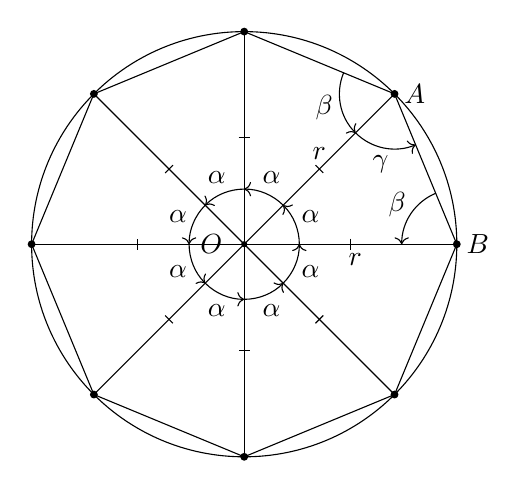
\begin{tikzpicture}[scale=1.0]

% parameters %{{{2

	\def\numsides{8}
	\def\radius{2.7}
	\def\rotation{90}

% coordinates %{{{2

	\coordinate (O) at (0,0);

	\foreach \i in {1,...,\numsides} {
		\coordinate (P\i) at ({360/\numsides*(\i-1)+\rotation}:\radius);
	}

% circle %{{{2

	\draw (O) circle (\radius);

% polygon %{{{2

	\draw (P1) \foreach \i in {2,...,\numsides} { -- (P\i) } -- cycle;

% radiuses %{{{2

	\foreach \i in {1,...,\numsides} { \draw (O) -- (P\i); }

% points, dots, vertices %{{{2

	\foreach \i in {1,...,\numsides} { \fill (P\i) circle (0.5mm); }

% points, dots, vertices labels %{{{2

	\node[label={[label distance=0.3mm]left:$O$}] at (O) {};
	\filldraw (O) circle (0.9pt);

	\node[right] at (P7) {$B$};
	\node[right] at (P8) {$A$};

	\node[above] at ($(O)!0.5!(P8)$) {$r$};
	\node[below left] at ($(O)!0.6!(P7)$) {$r$};

% segments marks %{{{2

	\foreach \i in {1,...,\numsides} {
		\tkzMarkSegments[mark=|, size=2pt](O,P\i)
	}

% angles labels %{{{2

	\foreach \i in {1,...,\numsides} {
		\pgfmathtruncatemacro{\j}{mod(\i,\numsides)+1}
		\ifodd\i
			\def\angradius{0.7cm}
		\else
			\def\angradius{0.7cm}
		\fi
		\pic[draw, ->, "$\alpha$", angle radius=\angradius, angle eccentricity=1.3]
		{angle = P\i--O--P\j};
	}

	\pic[draw, ->, "$\beta$", angle radius=0.7cm, angle eccentricity=1.3]
	{angle = P8--P7--O};

	\pic[draw, ->, "$\gamma$", angle radius=0.7cm, angle eccentricity=1.3]
	{angle = O--P8--P7};

	\pic[draw, ->, "$\beta$", angle radius=0.7cm, angle eccentricity=1.3]
	{angle = P1--P8--O};

% closing %{{{2

\end{tikzpicture}
\end{document}
